% Converted from README.md
\section{Ograničena provera modela (alat CBMC)}\label{ograniux10dena-provera-modela-alat-cbmc}

Provera modela je tehnika verifikacije softvera kojom se određuju sve moguće putanje kroz program i čuvaju u vidu konačnog automata. Zatim se prati svaka putanja i vrše se provere. Većina alata otkriva osnovne greške: deljenje nulom, mrtve petlje, trku za podacima itd.

Kod provere modela, program koji treba da se verifikuje je modelovan u vidu konačnog automata i specifikacija je zadata temporalnom logikom. Glavna ideja ograničene provere modela (engl. \emph{bounded model checking}) jeste da pronađe kontraprimer u izvršavanjima čija je dužina ograničena celim brojem \texttt{k}. Ako greška nije prijavljena, možemo povećavati \texttt{k} sve dok greška ne bude nađena, problem više ne može da se prati ili se dostigne neko drugo ranije definisano gornje ograničenje modela. Problem provere modela se efikasno može svesti na problem zadovoljivosti iskazne logike i kao takav može biti rešen SAT rešavačem. Moderni SAT rešavači rešavaju probleme i sa više stotina hiljada promenljivih.

Ograničena provera modela ima dve karakteristike:

\begin{itemize}
\tightlist
\item
  korisnik obezbeđuje ograničenje broja ciklusa koje treba istražiti, samim tim tehnika je nepotpuna ako je ograničenje nedovoljno visoko
\item
  koristi SAT tehnike.
\end{itemize}

Proverom modela automatski se pronalaze sve putanje koje se mogu izvršiti i čuvaju u internom modelu. Zatim se izvršava svaka putanja internog modela i proverava pojavljuju li se osnovne greške i da li su ispunjena svojstva modela. Svojstva modela se mogu zadati temporalnom logikom. Neki od operatora temporalne logike, za iskaze \texttt{p} i \texttt{q}:

\begin{itemize}
\tightlist
\item
  \texttt{Fp} - \texttt{p} važi neko vreme u budućnosti
\item
  \texttt{Gp} - \texttt{p} važi uvek u budućnosti
\item
  \texttt{Xp} - \texttt{p} važi sledeći put
\item
  \texttt{p} $\cup$ \texttt{q} - \texttt{p} važi dok \texttt{q} važi
\end{itemize}

Primer upotrebe operatora bi mogao da bude: Automobil ne kreće dok je menjač u poziciji \emph{Parking}.

\begin{minted}{text}
(~start) U gear_park
\end{minted}

\subsection{Primer sa mikrotalasnom rernom}\label{primer-sa-mikrotalasnom-rernom}

Uzmimo primer programa koji simulira rad mikrotalasne rerne. Svojstva koja moraju biti ispunjena:

\begin{itemize}
\tightlist
\item
  ako su vrata zatvorena, mogu biti otvorena.
\item
  ako su vrata otvorena, mogu buti zatvorena.
\item
  ako je grejač isključen, može biti uključen, ali samo ako su vrata zatvorena.
\item
  ako je grejač uključen, može biti isključen.
\end{itemize}

Ove zahteve možemo predstaviti programom:

\begin{minted}{java}
public class Microwave {
    boolean doorOpen = false;
    boolean heatOn = false;

    public Microwave() {}

    public void openDoor() {
        if (!doorOpen) doorOpen = true;
    }
 
    public void closeDoor() {
        if (doorOpen) doorOpen = false;
    }

    public void turnHeatOn() {
        if (!heatOn && !orOpen) heatOn = true;
    }

    public void turnHeatOff() {
        if (heatOn) heatOn = false;
    }
}
\end{minted}

Program dozvoljava otvaranje i zatvaranje vrata kao i paljenje i gašenje grejača. Kao zaštitno svojstvo, postoji provera da li su vrata zatvorena pre nego što se grejač uključi, inače ga neće uključiti. Kreirajmo konačni automat za ove funkcionalnosti:

\pandocbounded{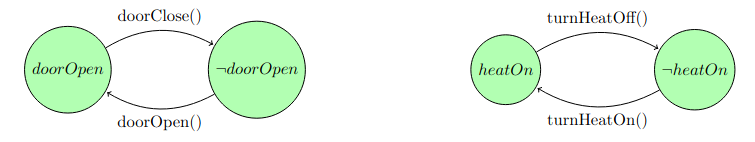
\includegraphics[keepaspectratio]{images/automata1.png}}

Dijagram na slici prikazuje kako se stanje program menja, tj. vrednosti promenljivih \texttt{doorOpen} i \texttt{heatOn}. Sastavimo kompletan dijagram:

\pandocbounded{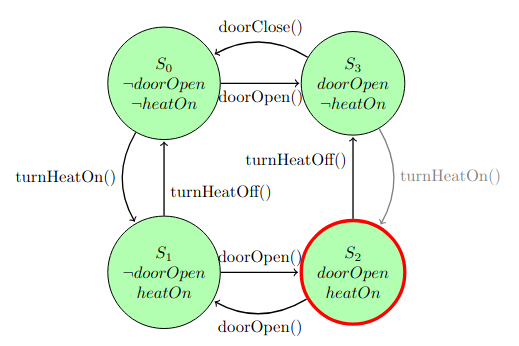
\includegraphics[keepaspectratio]{images/automata2.png}}

Na slici vidimo četiri stanja sa različitim vrednostima dve logičke promenljive u obliku krugova. Sistem može menjati stanje korišćenjem nekog od metoda klase. Imamo opasno stanje \texttt{S2} u kom su vrata otvorena i grejač uključen. U ovo stanje nije moguće doći pozivom metode \texttt{turnHeatOn()} iz stanja S3 jer je metoda tako napisana da ne uključuje grejač ako su vrata otvorena. Ipak, sistem može doći u sporno stanje \texttt{S2}, tako što prvo dođe u stanje \texttt{S1} i zatim pozove metod \texttt{doorOpen()} dok je grejač već uključen. Ta putanja možda nije uočljiva iz koda ili sa prvog automata. Međutim, postaje jasno vidljiva kada se napravi dijagram svih stanja.

Kada se kreira model programa i lista svojstava, moguće je ispratiti svaku moguću putanju i proveriti ispravnost svih svojstava.

U slučaju da promenljive programa mogu uzeti više vrednosti, bilo bi mnogo više stanja u modelu. Tada se koristi mnogo više memorije, pa možda i sva memorija na računaru. Ova pojava se zove eksplozija prostora stanja i to je i dalje aktivan problem za proveru modela.

Neki od alata za proveru modela shodno programskom jeziku:

\begin{itemize}
\tightlist
\item
  Java: NASA\textquotesingle s PathFinder, BANDERA, CBMC, DBRover
\item
  C/C++: BLAST, CBMC, PCAchecker, DBRover, DSVerifier, ESBMC, SATABS
\end{itemize}

\subsection{CBMC}\label{cbmc}

Alat \href{https://www.cprover.org/cbmc/}{CBMC}, kao i kompajleri, traži \texttt{.c} datoteku kao argument komandne linije. Prevodi program i objedinjuje ga sa definicijama drugih funkcija iz više \texttt{.c} datoteka, poput linkera. Ipak, umesto da proizvede izvršivu verziju programa, CBMC sprovodi simboličko izvršavanje programa.

\pandocbounded{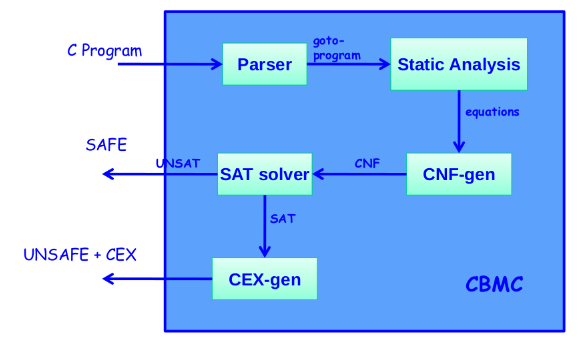
\includegraphics[keepaspectratio]{images/cbmc.png}}

\subsubsection{Primer sa argumentima komandne linije}\label{primer-sa-argumentima-komandne-linije}

Kao primer, razmotrimo program \texttt{01\_file1.c}:

\begin{minted}{c}
int puts(const char *s) { }

int main(int argc, char **argv) {
    puts(argv[2]);
}
\end{minted}

Očigledno je da program ima grešku, jer niz \texttt{argv} može imati i manje od 3 elementa i da se sa \texttt{argv{[}2{]}} izlazi izvan okvira niza. Pokrenimo CBMC sledećom komandom:

\begin{minted}{bash}
$ cbmc 01_file1.c --show-properties --bounds-check --pointer-check
\end{minted}

Opcije \texttt{-{}-bounds-check} i \texttt{-{}-pointer-check} navode CBMC da traži greške u vezi pokazivača ili granica nizova. Zbog opcije \texttt{-{}-show-properties} CBMC će štampati listu svih svojstava koje proverava. Prikazuje, između ostalog, i svojstvo \texttt{"object\ bounds\ in\ argv"} zajedno sa lokacijom pogrešnog pristupa elementu niza. CBMC uglavnom određuje svojstva koja treba da proveri. To se postiže preliminarnom statičkom analizom, koju vrši generator tvrđenja (engl. \emph{assertion generator}) \emph{goto-instrument} da označi deo koda koji potencijalno sadrži grešku.

Generator tvrđenja generiše tvrđenja za verifikaciju sledećih svojstava. Komande su izdvojene da bi se opcije mogle direktno kopirati u terminal:

\begin{itemize}
\tightlist
\item
  \textbf{Prekoračenje bafera} - Za svaki pristup elementu niza, proverava se da li je narušena donja ili gornja granica.
\begin{minted}{text}
--bounds-check
\end{minted}
\item
  \textbf{Upotreba pokazivača} - Traži dereferenciranje \texttt{NULL} ili neispravnih pokazivača.
\begin{minted}{text}
--pointer-check
\end{minted}
\item
  \textbf{Deljenje nulom} - Proverava da li u programu postoji deljenje nulom.
\begin{minted}{text}
--div-by-zero-check
\end{minted}
\item
  \textbf{Aritmetička potkoračenja i prekoračenja} - Proverava da li je došlo do prekoračenja ili potkoračenja prilikom aritmetičkih operacija nad označenim, neoznačenim ili realnim brojevima.
\begin{minted}{text}
--signed-overflow-check
--unsigned-overflow-check
--float-overflow-check
\end{minted}
\item
  \textbf{Nije broj} - Proverava da li račun sa realnim brojevima može da rezultuje \texttt{NaN} vrednošću.
\begin{minted}{text}
--nan-check
\end{minted}
\item
  \textbf{Neinicijalizovana promenljiva} - Proverava da li program koristi lokalnu promenljivu pre nego što je inicijalizovana.
\item
  \textbf{Trka za podacima} - Proverava da li dve niti programa pristupaju istoj deljenoj promenljivoj u isto vreme.
\end{itemize}

Daljom analizom je potrebno utvrditi da li su to zaista greške. CBMC sprovodi analizu simboličkom simulacijom, koja odgovara prevođenju programa u formulu. Ta formula se kombinuje sa svojstvom. Generisanu formulu možemo videti navođenjem opcije \texttt{-{}-show-vcc} (engl. \emph{Verification Condition}).

\begin{minted}{bash}
$ cbmc 01_file1.c --show-vcc --pointer-check
\end{minted}

Prilikom analize generiše se KNF formula koja opisuje program, zajedno sa svojstvima. To je izraz koji zadovoljava uslove problema i negaciju tvrđenja. Formula se prosleđuje SAT rešavaču koji odlučuje da li je formula zadovoljiva. Ako jeste, CBMC pronalazi kontraprimer. Ako nije, tvrđenje važi za izvršenje sa ograničenjem \texttt{k}.

Formula, odnosno uslovi verifikacije, treba tek da budu provereni da bi se proverilo da li važi navedeno svojstvo. Pokrećemo sa:

\begin{minted}{bash}
$ cbmc 01_file1.c --pointer-check
\end{minted}

Korišćenjem SAT rešavača, CBMC detektuje da ne važi uslov za granice niza \texttt{argv} i štampa sledeću poruku:

\begin{minted}{text}
Violated property:
  file 01_file1.c line 7 function main
  dereference failure: object bounds in argv[(signed long int)2]
\end{minted}

Da bismo razumeli problem i zašto svojstvo ne važi, CBMC može da nam generiše trag izvršavanja kontraprimera korišćenjem opcije \texttt{-{}-trace}:

\begin{minted}{bash}
$ cbmc 01_file1.c --pointer-check --trace
\end{minted}

Na ekranu nam se prikazuje kontraprimer, u vidu toka izvršavanja programa počevši od \texttt{main} funkcije do stanja koje narušava svojstvo. U ovom primeru svojstvo je narušeno u neispravnom indeksiranju elementa niza. Takođe, prikazuje nam i vrednosti koje ulazne promenljive treba da imaju da bi se izazvala greška. Prikazuje nam i uslov čijom proverom se došlo do zaključka.

\begin{minted}{text}
CBMC version 5.10 (cbmc-5.10) 64-bit x86_64 linux
Parsing 01_file1.c
Converting
Type-checking 01_file1
Generating GOTO Program
Adding CPROVER library (x86_64)
Removal of function pointers and virtual functions
Generic Property Instrumentation
Running with 8 object bits, 56 offset bits (default)
Starting Bounded Model Checking
size of program expression: 43 steps
simple slicing removed 10 assignments
Generated 7 VCC(s), 1 remaining after simplification
Passing problem to propositional reduction
converting SSA
Running propositional reduction
Post-processing
Solving with MiniSAT 2.2.1 with simplifier
462 variables, 1031 clauses
SAT checker: instance is SATISFIABLE
Solving with MiniSAT 2.2.1 with simplifier
462 variables, 0 clauses
SAT checker inconsistent: instance is UNSATISFIABLE
Runtime decision procedure: 0.00274368s

** Results:
[main.pointer_dereference.1] dereference failure: pointer NULL in argv[(signed long int)2]: SUCCESS
[main.pointer_dereference.2] dereference failure: pointer invalid in argv[(signed long int)2]: SUCCESS
[main.pointer_dereference.3] dereference failure: deallocated dynamic object in argv[(signed long int)2]: SUCCESS
[main.pointer_dereference.4] dereference failure: dead object in argv[(signed long int)2]: SUCCESS
[main.pointer_dereference.5] dereference failure: pointer outside dynamic object bounds in argv[(signed long int)2]: SUCCESS
[main.pointer_dereference.6] dereference failure: pointer outside object bounds in argv[(signed long int)2]: FAILURE
[main.pointer_dereference.7] dereference failure: invalid integer address in argv[(signed long int)2]: SUCCESS

Trace for main.pointer_dereference.6:

State 17  thread 0
----------------------------------------------------
    INPUT argc: 1 (00000000 00000000 00000000 00000001)

State 18  thread 0
----------------------------------------------------
    argv'[1]=((char *)NULL) (00000000 00000000 00000000 00000000 00000000 00000000 00000000 00000000)

State 21 file 01_file1.c line 3 thread 0
----------------------------------------------------
    argc=1 (00000000 00000000 00000000 00000001)

State 22 file 01_file1.c line 3 thread 0
----------------------------------------------------
    argv=argv' (00000010 00000000 00000000 00000000 00000000 00000000 00000000 00000000)

Violated property:
    file 01_file1.c line 5 function main
    dereference failure: pointer outside object bounds in argv[(signed long int)2]
    16l + POINTER_OFFSET(argv) >= 0l && OBJECT_SIZE(argv) >= 24ul + (unsigned long int)POINTER_OFFSET(argv) || DYNAMIC_OBJECT(argv)


** 1 of 7 failed (2 iterations)
VERIFICATION FAILED
\end{minted}

U ovom primeru, ako je \texttt{argc\ ==\ 1} dogodiće se prekoračenje granica niza \texttt{argv}. Ako dodamo proveru uslova da je \texttt{argc\ \textgreater{}=\ 3}, greška je otklonjena i CBMC-ov izveštaj dokazuje da su sva svojstva zadovoljena.

\subsubsection{Primer odvojenog testiranja funkcija}\label{primer-odvojenog-testiranja-funkcija}

CBMC je pisan sa namerom da se koristi i za ugrađen softver, a takvi programi obično imaju drugačije ulazne tačke od \texttt{main} funkcije. Pored toga CBMC je koristan za verifikaciju modula programa, poput ovog primera.

\begin{minted}{c}
int array[10];

int sum() {
    unsigned i, sum = 0;
    for (i = 0; i < 10; i++)
        sum += array[i];
}
\end{minted}

Potrebno je CBMC-u da naglasimo koja je ulazna tačka, a to je ovde funkcija \texttt{sum}. Pozivamo CBMC sa sledećim opcijama:

\begin{minted}{bash}
$ cbmc 02_file2.c --function sum --bounds-check
\end{minted}

Često je potrebno napraviti odgovarajuće propratne alate (\emph{eng. harness}) za funkciju da bi se podesilo odgovarajuće okruženje.

U ovom primeru možemo da primetimo i da CBMC odmotava petlju iz programa. Pošto CBMC formulu šalje SAT rešavaču, formula mora biti konačna. Zbog toga CBMC izvršava ograničenu proveru modela. Stoga se petljama broj iteracija mora ograničiti odozgo da bi se garantovalo pronalaženje grešaka. CBMC može proveriti da li je izvršeno dovoljno odmotavanja.

Svaka druga petlja (\texttt{for}, \texttt{do-while}) biće prezapisana u \texttt{while} petlju.

Treba znati da su globalne promenljive inicijalizovane pre izvršavanja date funkcije, što može dovesti do drugačijih stanja od onih prilikom realnog izvršavanja funkcije. CBMC ne pokušava da odredi preduslove za argumente funkcije.

\subsubsection{Primer neuspelog odmotavanja petlji}\label{primer-neuspelog-odmotavanja-petlji}

\begin{minted}{c}
int binsearch(int x) {
    int a[16];
    signed low = 0, high = 16;

    while (low < high) {
        signed middle = low + ((high - low) >> 1);

        if (a[middle] < x)
            high = middle;
        else if (a[middle] > x)
            low = middle + 1;
        else // a[middle] == x
            return middle;
    }

    return -1;
}
\end{minted}

Pokrenimo CBMC:

\begin{minted}{bash}
$ cbmc 03_binsearch.c --function binsearch --bounds-check
\end{minted}

Primetićemo da se odmotavanje petlje ne zaustavlja samo od sebe jer CBMC ne uspeva da otkrije gornje ograničenje za broj iteracija ove petlje. U tom slučaju gornje ograničenje za odmotavanje petlje mora da se zada preko opcije \texttt{-{}-unwind\ n}, gde \texttt{n} predstavlja broj provera uslova ostanka u petlji:

\begin{minted}{bash}
$ cbmc 03_binsearch.c --function binsearch --unwind 6  --bounds-check
\end{minted}

CBMC potvrđuje da su svi pristupi elementima niza u okviru granica, iako to u ovom slučaju zavisi od šiftovanja udesno. Ako se upotrebi opcija \texttt{-{}-unwinding-assertions}, proveravaće da li je petlja dovoljno odmotana. Za kraća odmotavanja od 6 bili bi ispisani koraci izvršavanja koji zahtevaju više odmotavanja petlje. Ako je pozvan i sa opcijom \texttt{-{}-trace}, generisaće nam i kontraprimer.

\begin{minted}{bash}
$ cbmc 03_binsearch.c --function binsearch --unwind 5 --unwinding-assertions  --bounds-check --trace
\end{minted}

\begin{minted}{text}
[binsearch.unwind.0] unwinding assertion loop 0: FAILURE

** 1 of 5 failed (2 iterations)
VERIFICATION FAILED
\end{minted}

\subsubsection{Primer sa neograničenim petljama}\label{primer-sa-neograniux10denim-petljama}

CBMC se može primeniti i na program sa neograničenim petljama. U takvim situacijama, CBMC služi samo za traženje grešaka i ne pokušava da pronađe sve. Program \texttt{04\_lock-example.c} je primer programa sa svojstvom koje je korisnik definisao, navodeći \texttt{assert} naredbe u kodu.

\texttt{while} petlja nema konkretnu gornju granicu broja iteracija. Stoga, mora se naglasiti koliko odmotavanja petlje treba CBMC da izvrši. Postoje dva načina da se tako nešto postigne:

\begin{itemize}
\tightlist
\item
  opcijom \texttt{-{}-unwind} da se ograniči koliko puta su petlje odmotane.
\item
  opcijom \texttt{-{}-depth} da se ograniči broj koraka programa koje treba pratiti.
\end{itemize}

Ukoliko navedemo i opciju \texttt{-{}-unwinding-assertions}, CBMC će proveriti da li je argument uz opciju \texttt{-{}-unwind} dovoljno veliki da pokrije sve putanje kroz program. Ukoliko je premali, detektovaće nam da nije izvršeno dovoljno odmotavanja.

Vratimo se na primer i pokrenimo CBMC:

\begin{minted}{bash}
$ cbmc 04_lock-example.c  --unwind 1 --unwinding-assertions
\end{minted}

Ne prijavljuje nam grešku, osim nedovoljnog odmotavanja. Ukoliko se izostavi poslednja opcija, neće ni to prijaviti. Već sa ograničenjem \texttt{2}, CBMC detektuje grešku. Upotrebom opcije \texttt{-{}-trace} generisaće se kontraprimer koji narušava važenje tvrđenja (\emph{eng. assertion}).

\begin{minted}{bash}
$ cbmc 04_lock-example.c  --unwind 1 --trace
\end{minted}

Bez prijave o nedovoljnom odmotavanju petlje ili korišćenjem opcije \texttt{-{}-depth}, CBMC ne dokazuje korektnost programa, ali je i dalje koristan za nalaženje grešaka.

Pokrećemo CBMC ponovo sa ciljem da proverimo ima li program grešaka.

\begin{minted}{bash}
$ cbmc 04_lock-example.c  --unwind 1
\end{minted}

Jedinu grešku koju dobijamo je da smatra da petlja nije odmotana do kraja. Zato pokrećemo ponovo sa većim brojem iteracija.

\begin{minted}{bash}
$ cbmc 04_lock-example.c  --unwind 2
\end{minted}

Dobijamo grešku da korisnikovo tvrđenje ne važi:

\begin{minted}{text}
** Results:
[lock.assertion.1] assertion !(LOCK != FALSE): SUCCESS
[unlock.assertion.1] assertion LOCK: FAILURE

** 1 of 2 failed (2 iterations)
VERIFICATION FAILED
\end{minted}

Generišimo i kontraprimer pozivom :

\begin{minted}{bash}
$ cbmc 04_lock-example.c  --unwind 2 --trace
\end{minted}

\begin{minted}{text}
Counterexample:

State 19 file lock-example.c line 19 function main thread 0
----------------------------------------------------
    got_lock=0 (00000000000000000000000000000000)

State 20 file lock-example.c line 19 function main thread 0
----------------------------------------------------
    got_lock=0 (00000000000000000000000000000000)

State 21 file lock-example.c line 20 function main thread 0
----------------------------------------------------
    times=1713006976 (01100110000110100110100110000000)

State 35 file lock-example.c line 32 function main thread 0
----------------------------------------------------
    got_lock=4294967295 (11111111111111111111111111111111)

State 36 file lock-example.c line 32 function main thread 0
----------------------------------------------------
    times=1713006975 (01100110000110100110100101111111)
\end{minted}

Shvatamo da se u toj jednoj iteraciji naše petlje dogodilo da je izvršena linija \texttt{32} i smanjena vrednost od \texttt{get\_lock}, a s obzirom da je tip \texttt{unsigned\ int}, dobila je vrednost najvećeg neoznačenog celog broja. To ne sme da se dogodi, jer je smisao te promenljive da se poveća kada se ostvari zaključavanje i da se smanji na \texttt{0} kada se otključa. Izmenimo kod i primetimo da više neće prijavljivati problem.

\subsubsection{Odmotavanje zasnovano na broju iteracija}\label{odmotavanje-zasnovano-na-broju-iteracija}

Pogledajmo primer \texttt{05\_loop1.c}

\begin{minted}{c}
int main(int argc, char **argv) {
    int i = 1;
    while (i < 5) {
        i = i + 1;
    }
    return 0;
}
\end{minted}

Ovo bi bio primer programa u kome je dovoljno da imamo 5 odmotavanja petlje. Transformisan program bez petlje izgleda ovako: \texttt{05\_loop1\_unwinded.c}

\codefile{examples/05_loop1_unwinded.c}{c}

Program odgovara toku izvršavanja petlje sa 4 iteracije, a uslov ostanka u petlji se 5 puta proverava. Odgovara pozivu:

\begin{minted}{bash}
$ cbmc 05_loop1.c  --unwind 5 --unwinding-assertions
\end{minted}

~Za svaki manji broj odmotavanja, manji od 5, prijavio bi nedovoljno odmotavanje. Transformisan kod za 3 odmotavanja bi izgledao ovako: \texttt{05\_loop1\_unwinded\_insufficently.c}

\codefile{examples/05_loop1_unwinded_insufficently.c}{c}

Odgovara pozivu:

\begin{minted}{bash}
$ cbmc 05_loop1.c  --unwind 2 --unwinding-assertions
\end{minted}

Ukoliko ograničimo odmotavanje petlje, i pri tom ne navedemo opciju \texttt{-{}-unwinding-assertions}, posle određenog broja iteracija pretpostaviće se da više ne važi uslov ostanka u petlji i nastaviće se dalje. Dakle, sve preostale putanje kroz petlju biće ignorisane.

\begin{minted}{c}
#include <assert.h>

int main(int argc, char **argv) {
    int i = 1;
    if (i < 5) {
        i = i + 1;
        if (i < 5) {
            i = i + 1;
            assume(!(i < 5));
        }
    }
}
\end{minted}

U mnogim slučajevima CBMC može da automatski odredi gornju granicu iteracija petlje, pa i u slučajevima kada broj odmotavanja petlje nije konstanta. Primer \texttt{06\_loop2.c} to prikazuje:

\codefile{examples/06_loop2.c}{c}

\texttt{while} petlja ima očigledno gornje ograničenje za broj iteracija, ali iz petlje se može i ranije izaći u zavisnosti od povratne vrednosti funkcije \texttt{f()}. CBMC može automatski da odmota petlju do završetka. To automatsko detektovanje granice odmotavanja petlji može biti neuspešno ukoliko broj iteracija petlje zavisi od podataka. Takođe, broj iteracija može biti prevelik ili neograničen. U tim slučajevima je bolje koristiti opciju komandne linije \texttt{-{}-unwind\ B}, gde \texttt{B} označava broj provera uslova ostanka u petlji, odnosno skokova na početak. Tada se telo petlje izvršava \texttt{B-1} put.

\subsubsection{Zadavanje ograničenja odmotavanja za pojedinačne petlje}\label{zadavanje-ograniux10denja-odmotavanja-za-pojedinaux10dne-petlje}

Upotrebom opcije \texttt{-{}-unwind} ograničenje za odmotavanje se namešta globalno, za sve petlje u programu. Pogledajmo primer \texttt{07\_loop3.c}:

\codefile{examples/07_loop3.c}{c}

Da bismo zadali ograničenje posebno za svaku petlju, prvo pokrenimo program sa opcijom \texttt{-{}-show-loops} da bismo dobili listu svih petlji u programu i njihove identifikatore.

\begin{minted}{bash}
$ cbmc 07_loop3.c --show-loops
\end{minted}

\begin{minted}{text}
CBMC version 5.10 (cbmc-5.10) 64-bit x86_64 linux
Parsing 07_loop3.c
Converting
Type-checking 07_loop3
Generating GOTO Program
Adding CPROVER library (x86_64)
Removal of function pointers and virtual functions
Generic Property Instrumentation
Loop main.0:
    file 07_loop3.c line 9 function main

Loop main.1:
    file 07_loop3.c line 13 function main
\end{minted}

Za program sa 2 petlje zadajemo ograničenja odmotavanja za petlje redom, 10, odnosno 20, opcijom \texttt{-{}-unwindset}.

\begin{minted}{bash}
$ cbmc 07_loop3.c --unwindset main.0:10,main.1:20 --unwinding-assertions
\end{minted}

\begin{minted}{text}
CBMC version 5.10 (cbmc-5.10) 64-bit x86_64 linux
Parsing 07_loop3.c
Converting
Type-checking 07_loop3
Generating GOTO Program
Adding CPROVER library (x86_64)
Removal of function pointers and virtual functions
Generic Property Instrumentation
Running with 8 object bits, 56 offset bits (default)
Starting Bounded Model Checking
Unwinding loop main.0 iteration 1 file 07_loop3.c line 9 function main thread 0
Unwinding loop main.0 iteration 2 file 07_loop3.c line 9 function main thread 0
Unwinding loop main.0 iteration 3 file 07_loop3.c line 9 function main thread 0
Unwinding loop main.0 iteration 4 file 07_loop3.c line 9 function main thread 0
Unwinding loop main.0 iteration 5 file 07_loop3.c line 9 function main thread 0
Unwinding loop main.0 iteration 6 file 07_loop3.c line 9 function main thread 0
Unwinding loop main.0 iteration 7 file 07_loop3.c line 9 function main thread 0
Unwinding loop main.0 iteration 8 file 07_loop3.c line 9 function main thread 0
Unwinding loop main.0 iteration 9 file 07_loop3.c line 9 function main thread 0
Not unwinding loop main.0 iteration 10 file 07_loop3.c line 9 function main thread 0
size of program expression: 140 steps
simple slicing removed 2 assignments
Generated 1 VCC(s), 1 remaining after simplification
Passing problem to propositional reduction
converting SSA
Running propositional reduction
Post-processing
Solving with MiniSAT 2.2.1 with simplifier
120 variables, 11 clauses
SAT checker: instance is SATISFIABLE
Solving with MiniSAT 2.2.1 with simplifier
120 variables, 0 clauses
SAT checker inconsistent: instance is UNSATISFIABLE
Runtime decision procedure: 0.00124571s

** Results:
[main.assertion.1] assertion i<100: SUCCESS
[main.unwind.0] unwinding assertion loop 0: FAILURE

** 1 of 2 failed (2 iterations)
VERIFICATION FAILED
\end{minted}

\subsubsection{Odsecanje petlji}\label{odsecanje-petlji}

U nekim slučajevima je poželjno da odsečemo veoma duboke petlje u cilju dostizanja koda koji dolazi posle petlje. Pogledajmo primer \texttt{08\_loop4.c}:

\codefile{examples/08_loop4.c}{c}

U ovom primeru za malo ograničenje odmotavanja petlje provera posle petlje neće biti izvršena. Ako se smatra da neka petlja nije bitna za kod koji sledi posle nje, možemo koristiti opciju \texttt{-{}-partial-loops}. Ova opcija dozvoljava da se delimično izvrše putanje kroz petlju i time i za mala ograničenja odmotavanja pronalazi kontraprimer za proveru koja se izvršava posle petlje.

\begin{minted}{bash}
$ cbmc 08_loop4.c  --unwind 1 --partial-loops
\end{minted}

Problem sa delimičnim izvršavanjem petlje je što putanja koja na kraju bude izvršena ne mora biti jedna od validnih putanja kroz petlju u originalnom programu. Opcijom \texttt{-{}-partial-loops} stavlja se \texttt{break} naredba na mestu gde stoji \texttt{assert}, odnosno \texttt{assume}, prilikom ograničenog odmotavanja petlje sa opcijom \texttt{-{}-unwinding-assertions}, odnosno bez nje.

Pozivom:

\begin{minted}{bash}
$ cbmc 08_loop4.c  --unwind 10
\end{minted}

se ne dolazi do provere \texttt{assert} i ne detektuje se greška. Potrebno je da se petlja razmota 10001 put, da bi se stiglo do ostatka programa.

\subsubsection{Odmotavanje zasnovano na dubini (Depth-based Unwinding)}\label{odmotavanje-zasnovano-na-dubini-depth-based-unwinding}

Ograničenje za broj odmotavanja petlje nekada nije dovoljno. U situacijama kada je teško kontrolisati veličinu generisane formule samo opcijom \texttt{-{}-unwind}, opcijom \texttt{-{}-depth\ D} zadajemo da je odmotavanje petlje ograničeno brojem instrukcija koje su izvršene na toj putanji, bez obzira na redni broj iteracije petlje. CBMC koristi broj instrukcija u grafu kontrole toka (\emph{eng. control flow graph}), a ne broj instrukcija u izvornom kodu.

\subsubsection{Dekompozicija koraka analize}\label{dekompozicija-koraka-analize}

Instrumentacija:

\begin{minted}{bash}
$ cbmc 09_abs.c --function abs --signed-overflow-check --show-goto-functions
\end{minted}

Svojstva:

\begin{minted}{bash}
$ cbmc 09_abs.c --function abs --signed-overflow-check --show-properties
\end{minted}

Static Single Assign (SSA):

\begin{minted}{bash}
$ cbmc 09_abs.c --function abs --signed-overflow-check --program-only
\end{minted}

Verification condition (VCC):

\begin{minted}{bash}
$ cbmc 09_abs.c --function abs --signed-overflow-check --show-vcc
\end{minted}

Verify:

\begin{minted}{bash}
$ cbmc 09_abs.c --function abs --signed-overflow-check
\end{minted}

\subsubsection{Uprošćavanje verifikacione formule}\label{uproux161ux107avanje-verifikacione-formule}

\begin{minted}{bash}
$ cbmc 10_escapefunction.c --function escape --pointer-check --bounds-check \
    --slice-formula --unwind 4
\end{minted}

Opcija \texttt{-{}-slice-formula} uklanja nepotrebne dodele, tj. dodele koje nisu u vezi sa svojstvima koje proveravamo. Na taj način uprošćava formulu koja se šalje SAT solveru i ubrzava proveru modela. Ispravimo prijavljene greške i proverimo ponovo. Nije moguće rešiti problem što \texttt{s} može biti bilo kakav pokazivač.

U programu \texttt{11\_escapefunctionharness.c} imamo \texttt{main} funkciju koja će adekvatno pripremiti sve argumente potrebne za funkciju \texttt{escape}.

\begin{minted}{bash}
$ cbmc 11_escapefunctionharness.c --pointer-check --bounds-check \
    --slice-formula --unwind 4
\end{minted}

Probati sa različitim ograničenjem za odmotavanje. Uočiti greške i ispraviti ih. Zatim povećati ograničenje radi pretrage drugih grešaka (\texttt{\textgreater{}20}).

\subsubsection{Binarna reprezentacija grafa kontrole toka}\label{binarna-reprezentacija-grafa-kontrole-toka}

\texttt{goto-cc} je CBMC-ova zamena za kompajler i linker, (\texttt{goto-cl} verzija za MS VisualStudio). Komandom

\begin{minted}{bash}
$ goto-cc 12_simple.c -o simple.goto
\end{minted}

dobijamo binarnu reprezentaciju grafa kontrole toka.

Da bismo generisali instrumentovan C kod, izvršavamo komandu:

\begin{minted}{bash}
$ goto-instrument --dump-c simple.goto out.c
\end{minted}

\texttt{goto-instrument} čita binarnu reprezentaciju grafa kontrole toka i primenjuje odgovarajuću statičku analizu. Kod je dopunjen proverama na mestu gde je uočena potencijalna greška. Zatim se čuva dopunjena binarna reprezentacija. Komanda:

\begin{minted}{bash}
$ goto-instrument simple.goto --show-properties
\end{minted}

daje sva uočena svojstva prilikom instrumentacije. Instrumentovan kod analiziramo CBMC-om, izvršavanjem:

\begin{minted}{bash}
$ cbmc out.c
\end{minted}

ili:

\begin{minted}{bash}
$ cbmc simple.goto
\end{minted}

\subsubsection{Modelovanje problema}\label{modelovanje-problema}

CBMC obezbeđuje primitive koje nisu pisane na jeziku C, a koje modeluju nedeterminističke funkcije, tj. funkcije koje mogu uzastopno vratiti mnogo različitih vrednosti. Upotreba:

\begin{minted}{c}
int nondeter_int();
\end{minted}

deklariše nedeterminističku funkciju koja vraća podatak tipa \texttt{int}. Ovakve funkcije su dostupne za razne tipove. Nedeterminističke funkcije su korisne prilikom modelovanja ulaznih podataka, nepoznatog okruženja, bibliotečkih funkcija i praktično bilo čega što se može različito ponašati prilikom izvršavanja u različitim okruženjima. Modelovanje nedeterminističkim funkcijama je praktično, ali može biti skupo. Sve moguće putanje izvršavanja moraju biti razmotane i istražene, čak i one koje nisu moguće u praksi.

CBMC omogućava eksplicitno zadavanje korisnikovih preduslova i postuslova i time omogućava da se analiza vrši po funkciji, čime se značajno smanjuje opterećenje analizatora. Da bismo proverili da li određeni poziv funkcije \texttt{foo} važi svojstvo \texttt{P}, delimo odlučivanje na dva dela:

\begin{itemize}
\tightlist
\item
  Pretpostavljajući da određeni predefinisani preduslov \texttt{C} važi u početnom stanju funkcije \texttt{foo}, i pretpostavljajući da svojstvo \texttt{P} važi na ulazu, da li svojstvo \texttt{P} važi i po izlasku iz funkcije?
\item
  Kad god je funkcija \texttt{foo} pozvana, da li garantovano važi preduslov \texttt{C} na ulazu?
\end{itemize}

Kada oba uslova važe, analiza će garantovano biti korektna. Na ovaj način se proveravaju samo preduslovi i postuslovi, ali ne i implementacija. Ovo olakšava testiranje, ali otvara prostor za sve potencijalne greške programera. Ponekad ima smisla kombinovati ovaj pristup sa klasičnom analizom. Na primer, u nekom programu se nedeterminističke funkcije koriste za modelovanje sistemskih poziva, dok se pretpostavke i garancije važenja uslova koriste na bibliotečkim funkcijama da bi osigurale njihovo izvršavanje i u isto vreme svele analizu kôda na manje, lokalne funkcije.

Tehnika postavljanja uslova i garancija važenja se postiže specifikacijom:

\begin{minted}{c}
__CPROVER_assert(uslov,poruka)
\end{minted}

Ovo je osnovni oblik korisnički definisanih specifikacija koje CBMC podržava. Kada se pokrene provera modela, proverava se važenje uslova navedenog kao prvi argument na svim putanjama do definisane granice. Ako granica nije data u komandnoj liniji, CBMC će kao i uvek pokušati da pronađe gornju granicu dubine izvršavanja programa i verifikovati ga nakon odmotavanja. Drugi argument je niska za dijagnostikovanje, jer će biti prikazana u rezultatu analize ako CBMC pronađe kontraprimer za uslov.

Pretpostavke okruženja se zadaju specifikacijom:

\begin{minted}{c}
__CPROVER_assume(uslov)
\end{minted}

CBMC interpretira ovaj poziv malo drugačije od prethodnog. Bilo koja putanja koja ne zadovoljava uslov naveden kao argument biće odbačena iz analize. Čak i ako takva putanja negde kasnije sadrži neku grešku, ona neće biti prijavljena u rezultatu. Ovo je korisno u slučajevima modelovanja okruženja, ukoliko verujemo da će argumenti prosleđeni funkciji uvek zadovoljavati navedene uslove. Ove dve specifikacije, zajedno sa nedeterminističkim funkcijama i programiranjem, omogućavaju modelovanje zanimljivih tvrđenja.

U primeru \texttt{05\_assume.c}, ne postoji izračunavanje za koje istovremeno može biti ispunjen uslov iz \texttt{if\ (\ x\textgreater{}0\ )} i pretpostavka iz \texttt{\_\_CPROVER\_assume\ (x\ \textless{}\ 0)}. Zbog svojstva \texttt{\_\_CPROVER\_assume} sve grane stabla izvršavanja od te pretpostavke koje ne zadovoljavaju uslov biće odbačene. Iz tog razloga CBMC neće prijaviti grešku, šta god uslov bio.

U primeru \texttt{06\_postcondition.c}, CBMC ne prijavljuje grešku iako za \texttt{N\ =\ -1} i \texttt{x\ =\ 0} ne bi važio uslov. To se događa jer \texttt{N} i \texttt{x} nisu inicijalizovane i CBMC pretpostavlja da su im vrednosti \texttt{0}. Da bismo uklonili tu pretpostavku moramo dodati nedeterminističke vrednosti za \texttt{N} i \texttt{x}.

\subsubsection{Višenitni programi}\label{viux161enitni-programi}

U primeru \texttt{10\_increment.c}, kontraprimer koji nam CBMC prijavljuje nam govori da je \texttt{x} dva puta postavljeno na 1. Problem je u pristupu kritičnoj sekciji od strane obe niti. Ograđivanjem kritične sekcije \texttt{mutex}-om rešavamo taj problem.

U primeru \texttt{11\_incrementLoop.c} problem je što imamo petlju u kojoj se čita vrednost deljene promenljive i potom ažurira. CBMC ne uspeva sam da odredi gornju granicu odmotavanja petlji, pa je neophodno da je zadamo.

U primeru \texttt{12\_mutex.c} postoje 3 niti, jedna glavna u kojoj se izvršava \texttt{main} funkcija, jedna koja je proizvođač (engl. \emph{producer}) i jedna koja je potrošač (engl. \emph{consumer}). Kako se program izvršava, instrukcije koje niti izvršavaju mogu se ukrstiti u bilo kom mogućem redosledu jer je raspoređivanje prepušteno operativnom sistemu. CBMC ovakve situacije modelira odmotavanjem kôda koji izvršava svaka nit u svim mogućim redosledima, tretirajući izbor rasporeda nedeterminističkim. Svaka nit ima svoj lokalni stek okvir, i on je dostupan samo odgovarajućoj niti. Globalne promenljive su dostupne svim nitima. Problem nastaje kada više niti pristupa deljenim podacima.

U ovom kodu \texttt{producer} i \texttt{consumer} pokušavaju da postignu međusobno isključenje preko 3 globalne promenljive: \texttt{try\_producer}, \texttt{try\_consumer} i \texttt{turn}. Kada bilo koja osim glavne niti želi da pristupi kritičnoj sekciji, ona signalizira svoju nameru postavljajući promenljivu \texttt{try\_producer}, odnosno \texttt{try\_consumer}, na 1. Potom daje priliku drugoj niti da uđe u kritičnu sekciju, postavljajući promenljivu \texttt{turn} na vrednost koja odgovara drugoj niti i čekajući u \texttt{while} petljama. Kada nit uđe u kritičnu sekciju, ona obavi svoj posao nad deljenim podacima i vraća vrednost promenljive \texttt{try\_producer}, odnosno \texttt{try\_consumer}, na 0.

Prvo ćemo ispraviti greške vezane za memoriju. Neki problemi sa memorijom mogu biti izazvani prilikom pristupanja deljenim podacima ako međusobno isključenje dve niti nije ispunjeno.

CBMC ne može naći gornju granicu odmotavanja petlji, naročito zato što imamo petlje u kojima niti čekaju na ulazak u kritičnu sekciju.

\begin{minted}{bash}
$ cbmc 12_mutex.c --unwind 7 --no-unwinding-assertions \
    --slice-formula --bounds-check --pointer-check
\end{minted}

Pronalazi nam kontraprimer u kom se vidi da nit koja odgovara funkciji \texttt{consumer} ulazi prva u kritičnu sekciju i svojom akcijom smanjuje \texttt{num\_waiting} na -1, a potom se poziva funkcija \texttt{process} da ispiše element na tom indeksu.

Ponavljamo prethodni poziv i iz podužeg kontraprimera zaključujemo da u poslednjoj liniji funkcije \texttt{next\_data} ne vraćamo vrednost koju smo upisali u niz, već narednu. Popravljamo funkciju tako da vrati vrednost na indeksu \texttt{data\_pos-1}.

Opcija komandne linije \texttt{-{}-unwind\ 7} utiče na međusobno isključenje niti, jer utiče na petlju u kojoj se čeka na dozvolu za ulazak u kritičnu sekciju. Petlja se izvršava kao da smo dodali \texttt{break} nakon 6. iteracije. Zbog toga se mogu dogoditi nejasne greške, na primer da \texttt{num\_waiting} bude smanjen na 0 u niti \texttt{consumer}, a potom vraćen na 2 u niti \texttt{producer}, što se ne bi smelo dogoditi.

Uveriti se da i \texttt{producer} i \texttt{consumer} nit završavaju i da su svi podaci iz \texttt{data\_source} obrađeni od strane niti \texttt{consumer}. Biće potrebno modifikovati kod da bi se ovo ostvarilo. Savet je da se koriste CBMC-ove korisničke specifikacije.
